% !TEX program = xelatex
% =============================================================
% 数维杯 / 中文赛道 论文骨架（ctexart 版式）
% 编译：latexmk -pdfxe main_zh.tex   或  .\build.ps1 -Target zh
% 若官方给的是 cumcmthesis.cls（国赛模板），把下面 \documentclass 换掉即可，
% 正文结构不用动；本机缺 cumcmthesis.cls，需手动放入模板目录。
% =============================================================
\documentclass[UTF8, zihao=-4, fontset=windows, a4paper]{ctexart}

\usepackage[a4paper,margin=2.5cm,headheight=15pt]{geometry}
\usepackage{amsmath,amssymb,bm,mathtools}
\usepackage{booktabs,tabularx,multirow,longtable,array}
\usepackage{graphicx}
\usepackage{listings}
\usepackage{siunitx}
\usepackage{pgfplots}
\pgfplotsset{compat=1.18}
\usepackage[ruled,vlined,linesnumbered]{algorithm2e}
\usepackage{subcaption}
\usepackage{tikz}
\usetikzlibrary{arrows.meta,positioning}
\usepackage{enumitem}
\usepackage{fancyhdr}
% 参考文献：MiKTeX 25.12 的 bibtex 遇到中文 .aux 会崩(0xC0000374)，改用 biber
\usepackage[backend=biber,style=gb7714-2015]{biblatex}
\addbibresource{refs.bib}
\usepackage{caption}
\captionsetup{font=small,labelsep=quad}
\usepackage{xcolor}
\usepackage[hidelinks,bookmarksnumbered]{hyperref}
\usepackage{microtype}

\ctexset{
  section     = {format = \Large\bfseries, number = \chinese{section}, aftername = {、}},
  subsection  = {format = \large\bfseries},
}
\newcommand{\todo}[1]{\textcolor{red}{[#1]}}   % 赛时删除全部 \todo{}
\pagestyle{fancy}
\fancyhf{}
\fancyhead[C]{\small 数维杯大学生数学建模竞赛}
\fancyfoot[C]{\small \thepage}
\renewcommand{\headrulewidth}{0.4pt}

\title{\todo{论文标题：名词化短标题，20 字以内}}
\author{\todo{队号 / 学校}}
\date{}

\begin{document}
\maketitle

% ============================ 摘要 ============================
\begin{center}
  \textbf{\large 摘\quad 要}
\end{center}

\todo{摘要写法（评委只看这一页也要能判分）：第一段交代问题与目标；
第二段写“建了什么模型、变量是什么、约束是什么”；第三段写“怎么求解”；
第四段放三个带具体数字的结论；最后一句写模型价值与适用边界。全文不写公式、不引文献。}

针对\todo{问题背景}，本文建立\todo{模型名称}。首先，\todo{数据预处理与特征}；
其次，以\todo{决策变量}为对象，构建\todo{目标函数与约束}；
最后，采用\todo{求解算法}求解，并用\todo{方法}检验稳健性。

结果表明：\todo{结论 1（含数字）}；\todo{结论 2（含数字）}；
\todo{结论 3（含数字）}。灵敏度分析显示\todo{参数在何范围内结论不变}。

\vspace{0.6em}
\noindent\textbf{关键词：}\todo{关键词1；关键词2；关键词3；关键词4}

\newpage
% ============================ 一、问题重述 ============================
\section{问题重述}

\subsection{问题背景}
\todo{3--5 段，每段一个意思：背景 → 现状做法 → 缺口 → 需要什么模型。}

\subsection{问题提出}
题目要求我们：
\begin{enumerate}[label=（\arabic*）,leftmargin=2.8em]
  \item \todo{问题一要求……}
  \item \todo{问题二要求……}
  \item \todo{问题三要求……}
\end{enumerate}

% ============================ 二、模型假设 ============================
\section{模型假设}
\begin{enumerate}[label=\textbf{假设\arabic*：},leftmargin=4.2em]
  \item \todo{假设表述。} \todo{合理性论证：数据支撑 / 量纲分析 / 文献依据。}
  \item \todo{假设表述。} \todo{若不成立会怎样。}
\end{enumerate}

% ============================ 三、符号说明 ============================
\section{符号说明}
\begin{table}[htbp]
  \centering
  \caption{主要符号说明}
  \label{tab:notation}
  \begin{tabular}{@{}lll@{}}
    \toprule
    符号 & 含义 & 单位 \\
    \midrule
    $x_{i}$    & \todo{决策变量}   & \si{\metre} \\
    $c_{ij}$   & \todo{成本系数}   & 元 \\
    $\theta$   & \todo{模型参数}   & -- \\
    $J(\cdot)$ & 目标函数          & -- \\
    \bottomrule
  \end{tabular}
\end{table}

% ============================ 四、模型建立与求解 ============================
\section{模型建立与求解}

\subsection{模型建立}
记 $\mathcal{I}$ 为\todo{对象集合}，决策变量 $x_i$ 表示\todo{含义}，建立
\begin{equation}
  \min_{x}\; J(x)=\sum_{i\in\mathcal{I}} c_{i}x_{i}
      +\lambda\sum_{i<j} w_{ij}\,\lvert x_{i}-x_{j}\rvert ,
  \label{eq:obj}
\end{equation}
约束为
\begin{align}
  \sum_{i\in\mathcal{I}} a_{i}x_{i} &\le b, \label{eq:cap}\\
  x_{i} &\ge 0,\quad x_{i}\in\mathbb{Z}\ (i\in\mathcal{I}_{d}),
  \label{eq:int}
\end{align}
其中 $\lambda\ge0$ 权衡\todo{效率与均衡}，式~\eqref{eq:cap} 刻画\todo{关键资源约束}；
整数约束的凸松弛处理参见\cite{boyd2004convex}。

\subsection{求解流程}
求解流程见图~\ref{fig:pipeline}。内层线性规划采用 HiGHS 的对偶单纯形实现
\cite{huangfu2018parallelizing}，外层搜索采用精英保留策略\cite{deb2002nsga2}。

\begin{figure}[htbp]
  \centering
  \begin{tikzpicture}[
      node distance=6mm and 9mm,
      box/.style={draw,rounded corners=1.5pt,align=center,
                  minimum height=7.5mm,inner sep=3pt,font=\small},
      ar/.style={-{Latex[length=1.6mm]},thick}]
    \node[box] (d) {数据\\预处理};
    \node[box, right=of d] (f) {特征\\构建};
    \node[box, right=of f] (m) {模型\\式~\eqref{eq:obj}};
    \node[box, right=of m] (s) {求解\\算法~\ref{alg:solve}};
    \node[box, right=of s] (v) {检验与\\灵敏度};
    \draw[ar] (d)--(f); \draw[ar] (f)--(m); \draw[ar] (m)--(s); \draw[ar] (s)--(v);
    \draw[ar, dashed] (v.south) -- ++(0,-5mm) -| (m.south);
  \end{tikzpicture}
  \caption{求解流程图（\todo{正文必须引用并解释一句}）}
  \label{fig:pipeline}
\end{figure}

\begin{algorithm}[htbp]
  \caption{混合搜索算法}\label{alg:solve}
  \KwIn{实例 $\mathcal{I}$，预算 $b$，种群规模 $N$，迭代代数 $G$}
  \KwOut{最优可行解 $x^{*}$}
  初始化种群 $\mathcal{P}\leftarrow\{x^{(1)},\dots,x^{(N)}\}$\;
  \For{$g=1$ \KwTo $G$}{
    按式~\eqref{eq:obj}--\eqref{eq:int} 评价 $J$\;
    锦标赛选择父代；交叉与变异\;
    对不可行子代按\todo{修复规则}修复\;
  }
  \Return{$\arg\min_{x\in\mathcal{P}} J(x)$}\;
\end{algorithm}

% ============================ 五、结果与分析 ============================
\section{结果与分析}

\subsection{主要结果}
表~\ref{tab:main} 给出与\todo{基线}的对比。

\begin{table}[htbp]
  \centering
  \caption{\todo{数据集}/\todo{场景}上的结果对比}
  \label{tab:main}
  \begin{tabular}{@{}lS[table-format=2.3]S[table-format=2.3]S[table-format=1.1]@{}}
    \toprule
    方法 & {指标一} & {指标二} & {耗时/s} \\
    \midrule
    基线              & 12.400 & 0.910 & 8.2 \\
    \todo{本文(v1)}   & 15.700 & 0.945 & 6.4 \\
    \todo{本文(完整)} & 18.300 & 0.968 & 4.9 \\
    \bottomrule
  \end{tabular}
\end{table}

\begin{figure}[htbp]
  \centering
  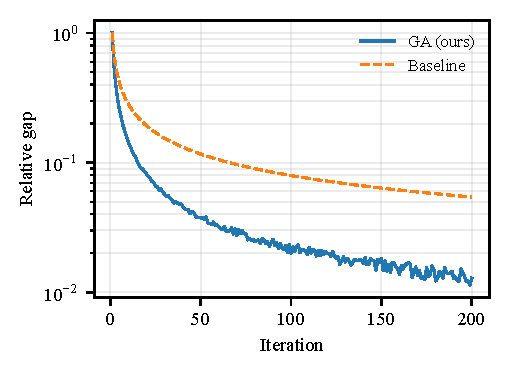
\includegraphics[width=0.62\linewidth]{figures/fig_convergence.pdf}
  \caption{算法收敛曲线（\todo{替换为真实结果}）}
  \label{fig:conv}
\end{figure}

\subsection{结果讨论}
\todo{不要复述表格。每段回答一个问题：为什么快、快在哪里、代价是什么；
用因果讲机制，避免“效果较好”这类空话。}

% ============================ 六、灵敏度分析 ============================
\section{灵敏度分析}
令 $\theta$ 在\todo{区间}内变动并重解（单因子设计，方法参见\cite{saltelli2008global}），
图~\ref{fig:sens} 显示目标值变化不超过
\todo{x\%}，\todo{排序何时反转}，说明\todo{结论稳健/脆弱}。

\begin{figure}[htbp]
  \centering
  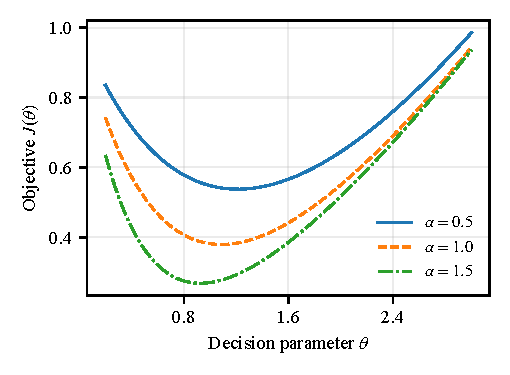
\includegraphics[width=0.62\linewidth]{figures/fig_sensitivity.pdf}
  \caption{目标函数随决策参数的变化（\todo{替换为真实结果}）}
  \label{fig:sens}
\end{figure}

% ============================ 七、模型评价与推广 ============================
\section{模型评价与推广}
\subsection{模型优点}
\begin{itemize}
  \item \todo{优点必须挂在一个结果上，不要形容词。}
  \item \todo{可解释性 / 可推广性。}
\end{itemize}
\subsection{模型缺点与改进}
\begin{itemize}
  \item \todo{缺点 + 对应的具体改进方案。}
\end{itemize}

% ============================ 八、结论 ============================
\section{结论}
\todo{4--6 句：回到问题、给最终数值结论、说明适用边界。不引入新内容。}

% ============================ 参考文献 ============================
\printbibliography[heading=bibintoc,title={参考文献}]

\newpage
\appendix
\section{核心代码}
\lstset{basicstyle=\ttfamily\footnotesize,breaklines=true,frame=single,
        numbers=left,numberstyle=\tiny}
\begin{lstlisting}[language=Python,caption={求解核心代码（节选）}]
import numpy as np
from scipy.optimize import milp, LinearConstraint, Bounds

def solve(c, A, b, integer_mask):
    res = milp(c=c, constraints=LinearConstraint(A, -np.inf, b),
               integrality=integer_mask.astype(int),
               bounds=Bounds(0, np.inf))
    return res.x, res.fun
\end{lstlisting}

\end{document}